\paragraph{Planning between the landmarks with no negative constraints}
\begin{figure}
    \centering
    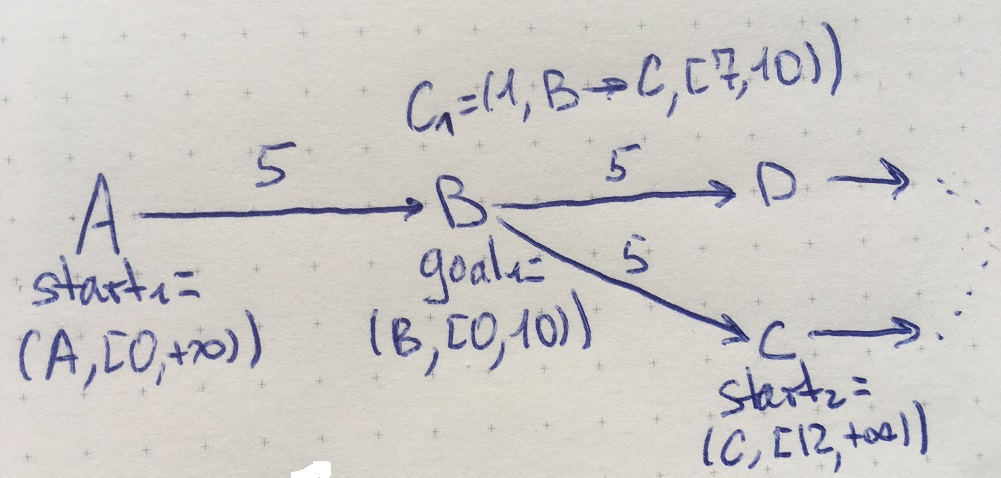
\includegraphics[width=\columnwidth]{Example_trimming_intervals.jpeg}
    \caption{Converting the time intervals of the positive constraint to \sipp's start and goal nodes (when no negative constraints are present).}
    \label{fig:trimming_intervals}
\end{figure}


Assume that only positive constraints are imposed on the agent $i$ and they define the following landmarks: $l_1=(i, a_1, [t_1,t_1'))$, ..., $l_k=(i, a_k, [t_k,t_k'))$. 

We, first, convert these landmarks to the sub-goals that \sipp has to consequently achieve: $goal_i=(from(a_i), [0, t_i'))$, where $from(a_i)$ denotes the source graph vertex of the action $a_i$. Please note, that the interval of $goal_i$ starts at $0$, not $t_i$. The rationale behind this is that the agent might arrive to $from(a_i)$ earlier than $t_i$ (and will often do so as \sipp reaches each state at the earliest possible time to guarantee optimality) and simply wait at $from(a_i)$ until $t_i$ (recall that no negative constraints that prohibit waiting at any graph vertex exist). This is a valid way of reaching $goal_i$.

Fig.~\ref{fig:trimming_intervals} shows an example of such trimming. Here the interval of the positive constraint $C_1$ is $[7, 10)$. However an agent might arrive to $B$ at time moment 5, wait at $B$ until time moment 7 comes and then start moving to $C$ satisfying the $C_1$. To account for this, the interval of $goal_1$ starts from 0 rather than from 7.

Time intervals of the intermediate start nodes are estimated in the following fashion. Assume that \sipp finishes its search to $goal_i$ arriving to it at $t_i^* < t_i'$, which is the earliest possible time $from(a_i)$ might be reached. The start node for the consecutive search, $start_{i+1}$, is defined now as $start_{i+1}=(to(a_i), [max(t_i, t_i^*) + d(a_i), \infty))$. Here $to(a_i)$ is the target vertex of the action $a_i$ and $d(\cdot)$ is the duration of an action. The interval of $start_{i+1}$ begins with the earliest possible time an agent can reach $to(a_i)$ via the landmark $l_i$ and spans till infinity as no negative constraints are present.

In case depicted on Fig.~\ref{fig:trimming_intervals} an agent arrives to $goal_1$ at 5, thus $t_1^*=5$. The interval of the positive constraint $C_1$ starts with 7, thus $t_1=7$. Indeed, $max(t_1^*, t_1)=7$ and the duration of $B \rightarrow C$ is 5. So the interval of $start_2$ begins with $12=7+5$.

In general, when only positive constraints are present, defining the intervals of start and goal nodes for sequential invocation of an individual planner is straightforward (as described above). However, when negative constraints exist, their time intervals might interfere with the landmarks in a more involved way resulting in necessity to define multiple start/goal nodes and plan between them.

\roni{I couldn't follow how this works from the text. A pseudo-code would be good.}
\konstantin{I added an example. Did it make the thing clearer?}